\documentclass[11pt,a4paper, twocolumn]{article}
\usepackage[T1]{fontenc}
\usepackage[utf8]{inputenc} % para poder usar tildes en archivos UTF-8
\usepackage[spanish]{babel} % para que comandos como \today den el resultado en castellano
\usepackage{a4wide} % márgenes un poco más anchos que lo usual
\usepackage[sinEntregas]{caratula}
\usepackage{float} 
\usepackage[section]{placeins}  
\usepackage{enumerate}

%\usepackage{helvet}

\begin{document}

\titulo{Trabajo Práctico 02}
\subtitulo{Informe}

\fecha{\today}

\materia{Laboratorio de Datos}
\grupo{EcuJaRu2}

\integrante{Fomina, Evangelina}{520/23}{evangelina.miloslav9@gmail.com}
\integrante{Niikado, Marina}{711/07}{niikadomarina@gmail.com}
\integrante{Borja, Kurt}{695/19}{kuurtb@gmail.com}
% Pongan cuantos integrantes quieran
\onecolumn

\maketitle

%\twocolumn

%\section{Resumen}
\section{Introducción}

El objetivo de este trabajo práctico es desarrollar dos modelos de clasificación de letras mayúsculas escritas a mano, uno para las letras ``A'' y ``L'' y otro para todas las vocales del alfabeto latino. Usando los métodos de aprendizaje automático supervisado \textbf{k-nearest neighbors} (\textbf{k-NN}) y \textbf{decision tree} respectivamente.

Para esto contamos con una versión reducida del popular dataset EMNIST (Cohen et al., 2017), que incluye solo las letras mayúsculas del alfabeto inglés. Viene dado como una matriz cuyas columnas representan el valor del canal alpha de cada píxel de una imagen de tamaño $28 \times 28$, junto con un label (785 columnas) y cuyas filas son cada elemento de la muestra. Este cuenta con 26 clases (una para cada letra) y una muestra de 2400 letras escritas a mano para cada clase, en total 62400 elementos balanceados.

A continuación, en lo que resta de la sección, los valores de los píxeles serán escalados con el método \textit{min-max}.

\begin{figure}[H]
	\centering
	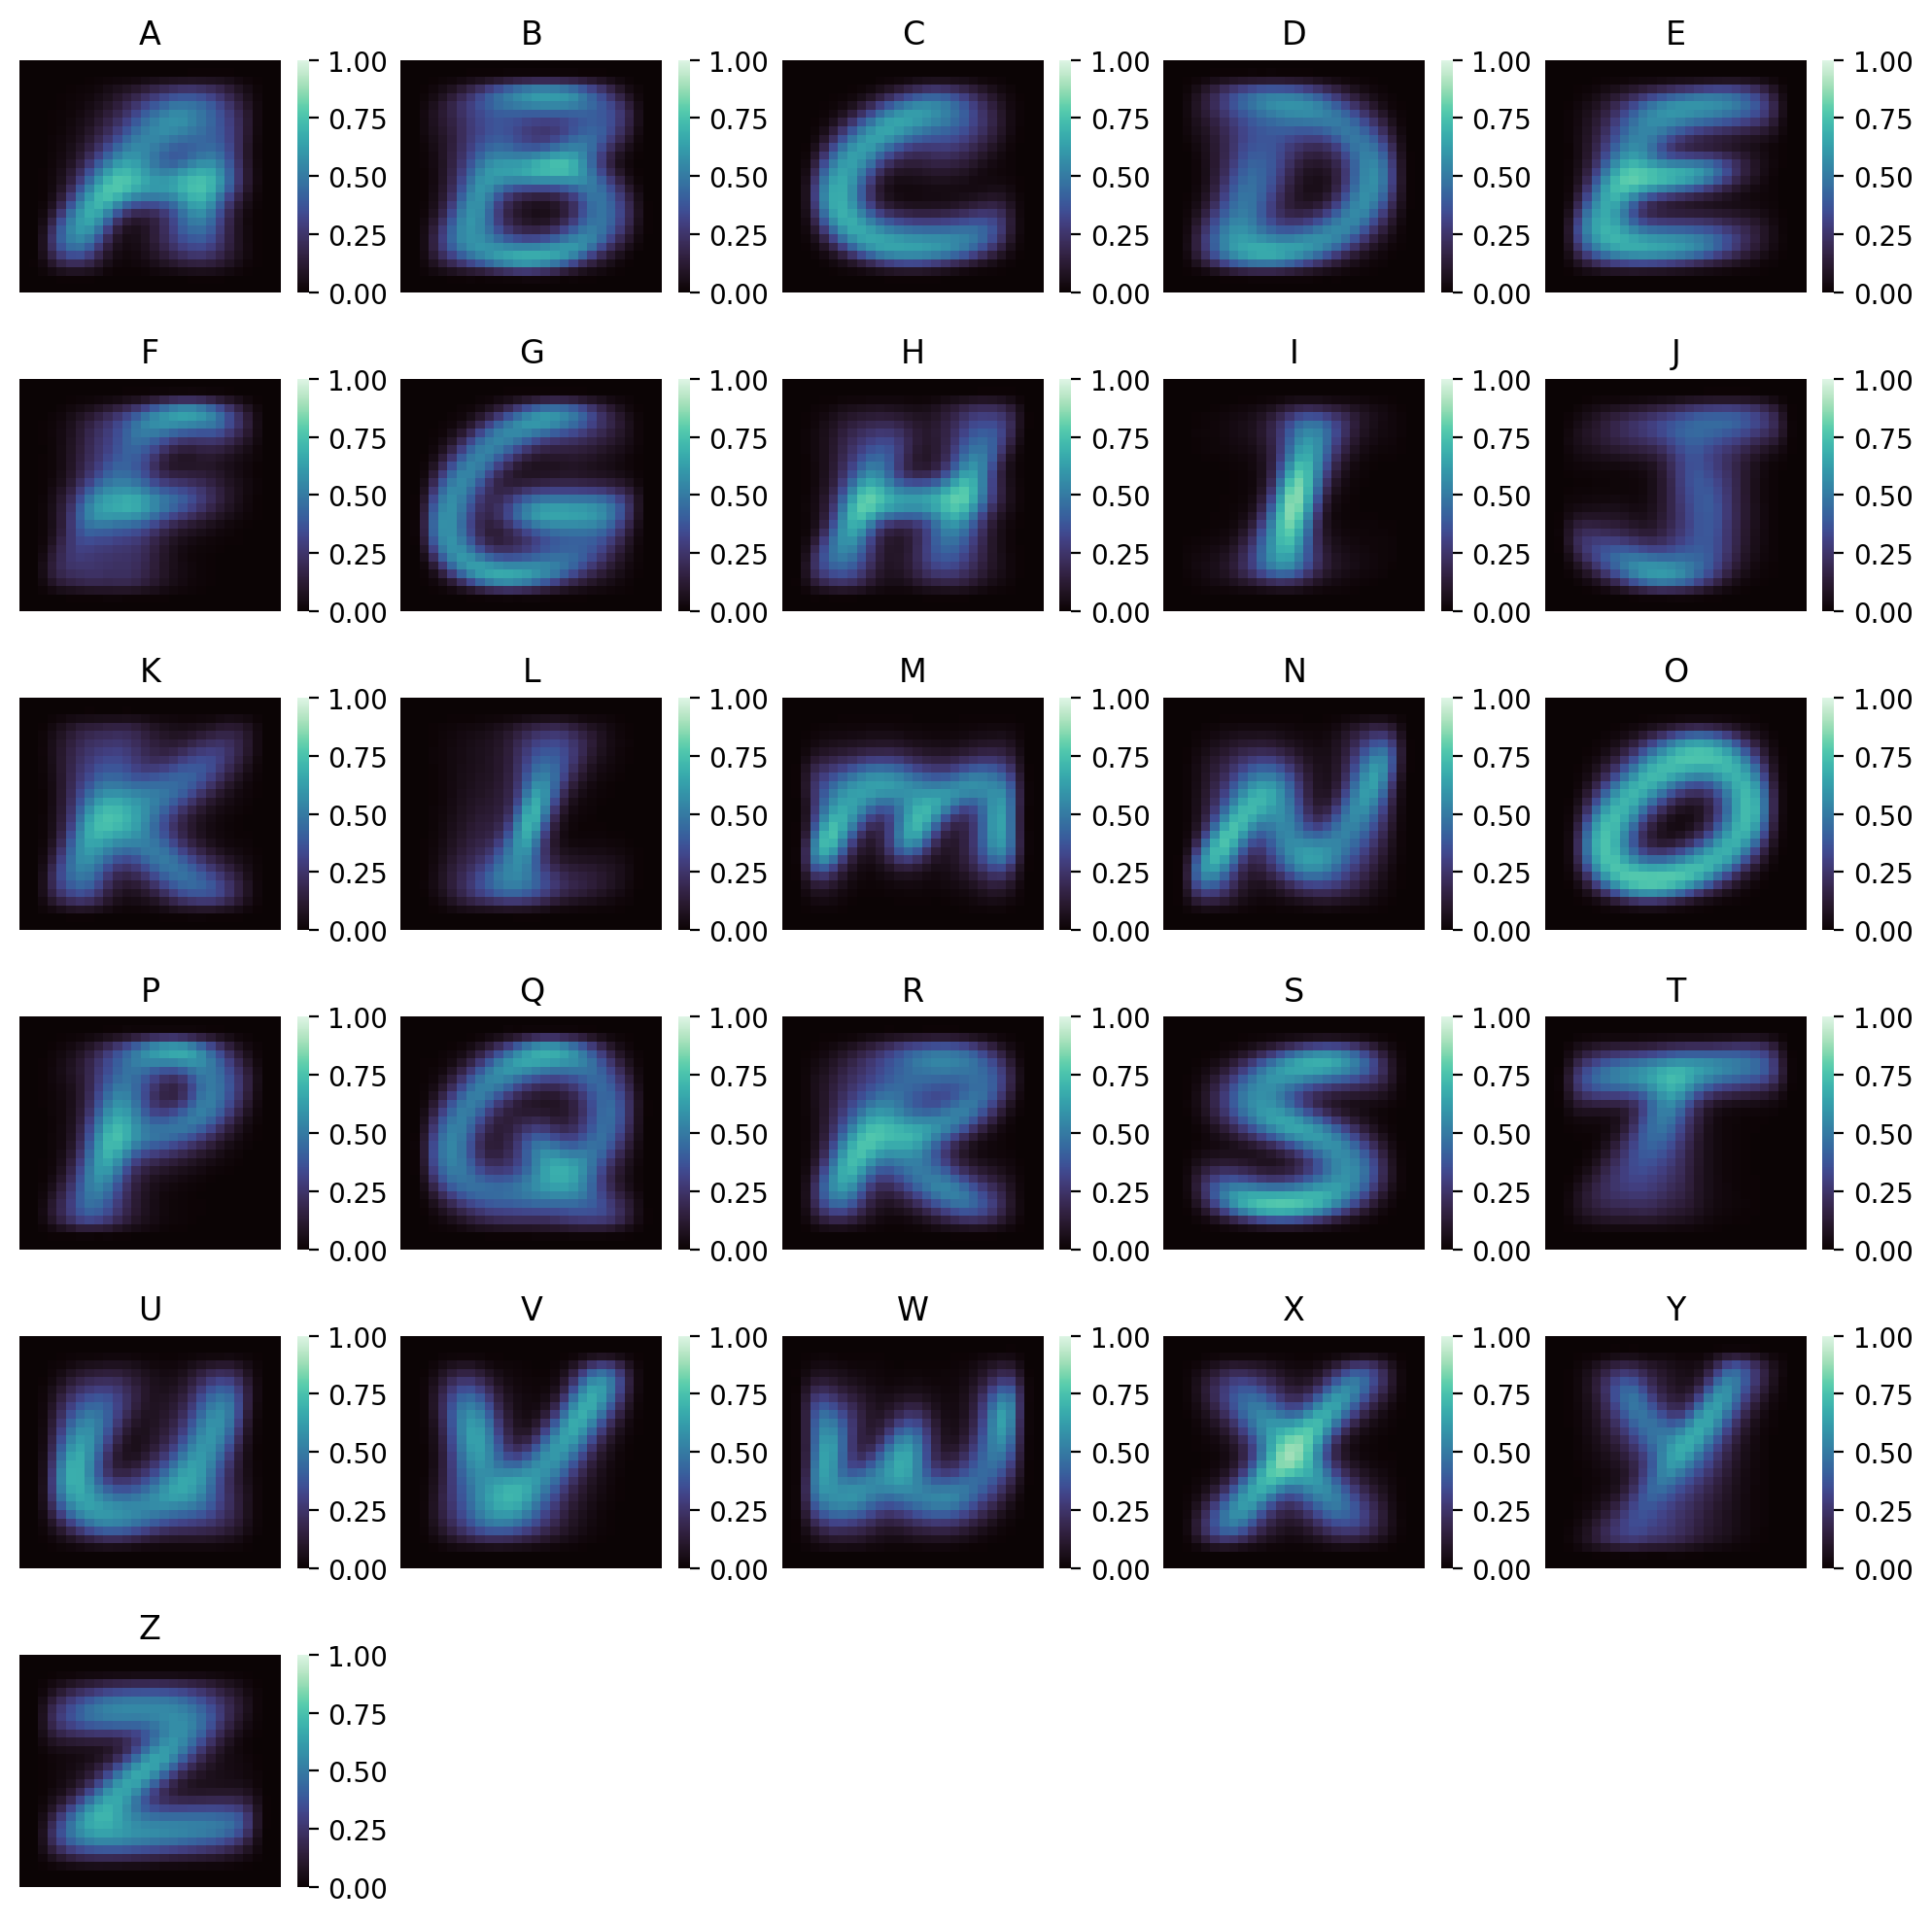
\includegraphics[scale=0.5]{figuras/1a.png}
	\caption{Media de cada parámetro para cada clase.}
	\label{fig:1a}
\end{figure}

Con el propósito de reducir la complejidad de nuestros modelos, para seleccionar los atributos más relevantes, tomamos la media de cada parámetro por clase, como se observa en la Figura \ref{fig:1a}. Luego, tomamos la desviación estándar de cada pixel de estas medias como se observa en la Figura \ref{fig:2a}.

\begin{figure}[H]

	\centering
	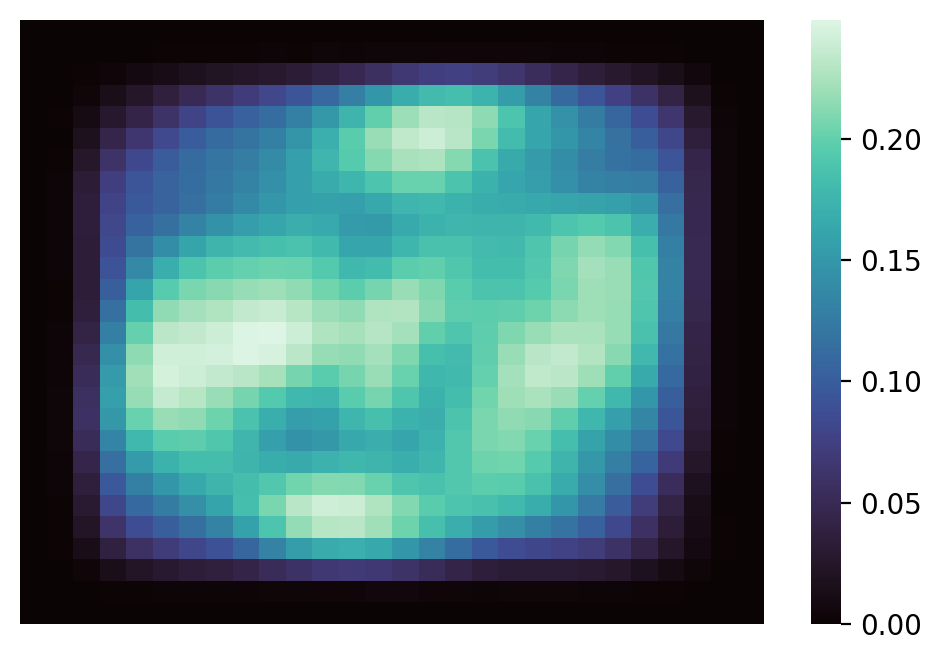
\includegraphics[scale=0.8]{figuras/2a.png}
	\caption{Desviación estandar entre la media de todas las clases.}
	\label{fig:2a}
\end{figure}

Nuestra hipótesis es que las variables con más desviación estándar entre clases, codifican más información sobre éstas. Como nuestros modelos van a ser entrenados sobre un subconjunto de estas clases, tomamos las más relevantes para nuestro objetivo, como se ve en la Figura \ref{fig:3a}.

\begin{figure}[H]
	\centering
	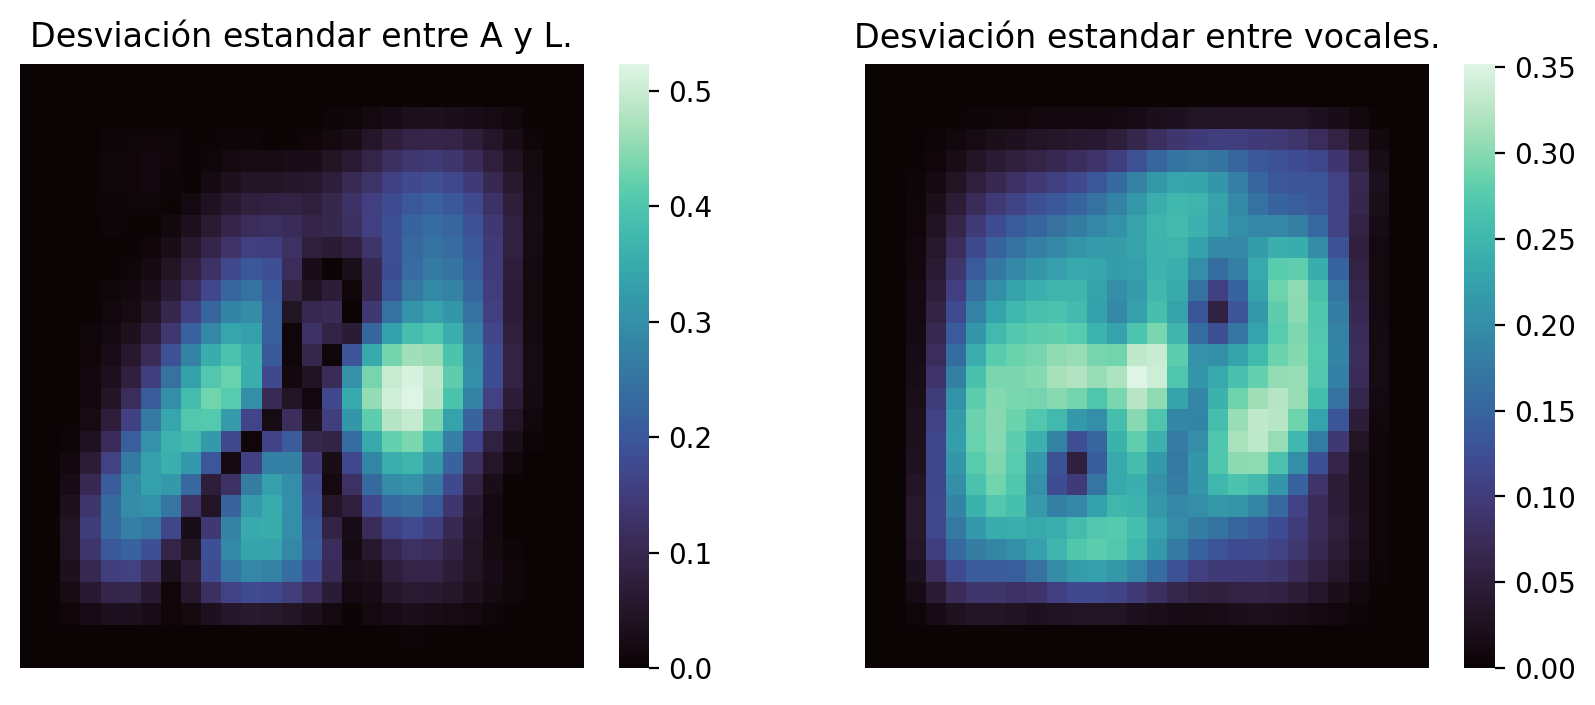
\includegraphics[scale=0.7]{figuras/3a.png}
	\caption{Desviación estándar entre la media de clases relevantes.}
	\label{fig:3a}
\end{figure}

Luego, para analizar qué tanto se parecen dos clases entre sí tomamos el coeficiente de correlación de Pearson entre las medias de cada clase. Por ejemplo las letras ``E'' y ``L'' tienen un coeficiente de correlación de $\approx 0.64$ a comparación de las letras ``E'' y ``M'' que tienen un coeficiente de correlación de $\approx 0.41$. Estos resultados son intuitivos ya que las letras ``E'' y ``L'' comparten trazos. En la Figura \ref{fig:4a} vemos el coeficiente de correlación para todos los posibles pares de letras.

\begin{figure}[H]
	\centering
	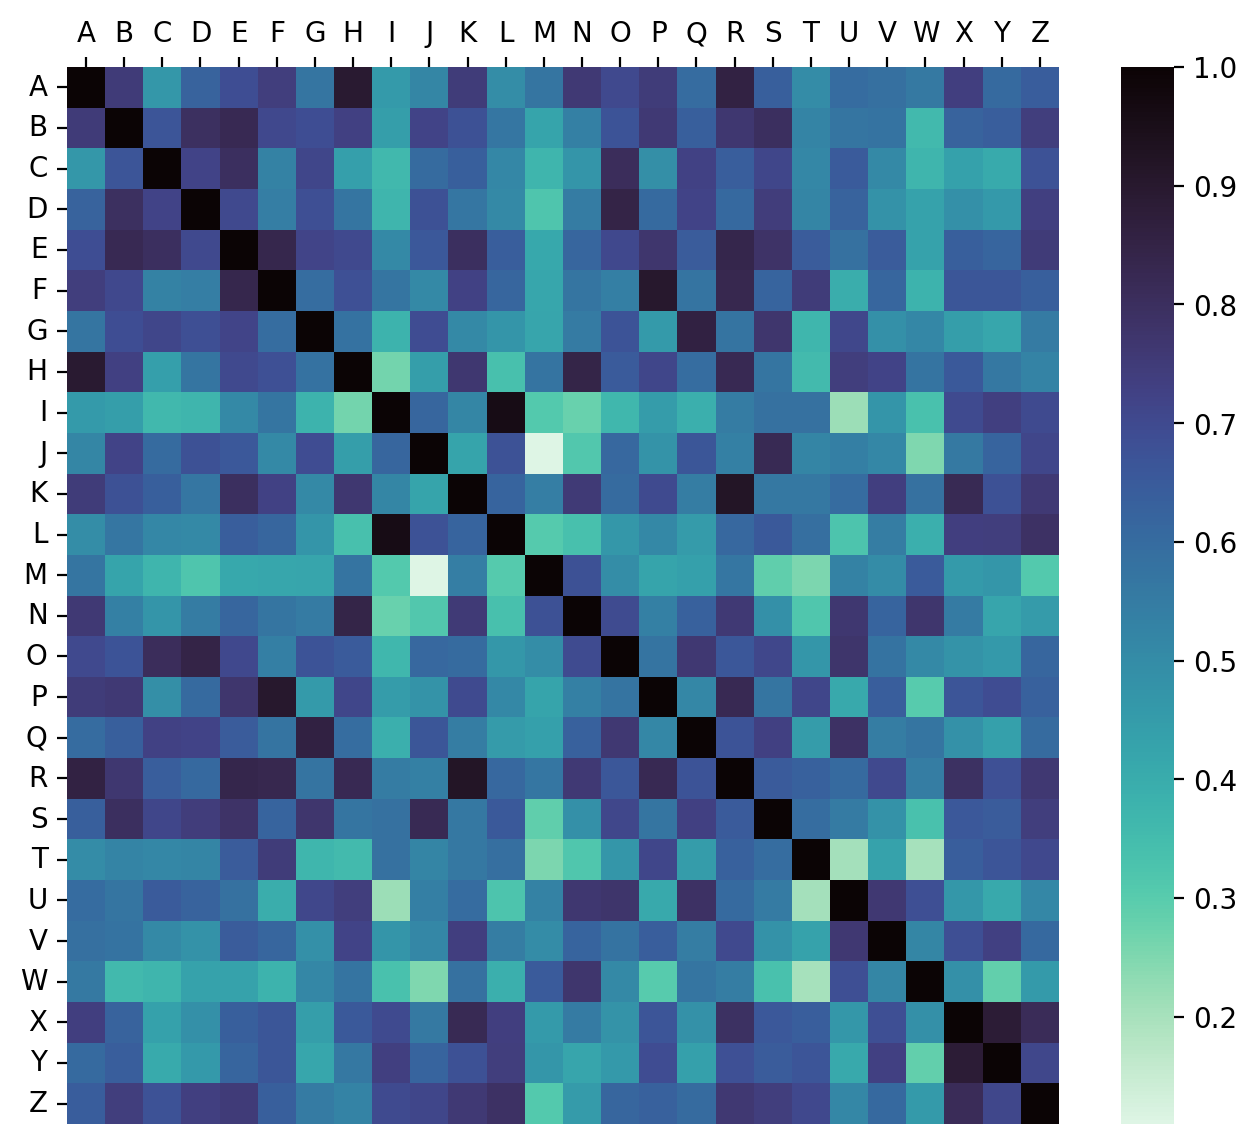
\includegraphics[scale=0.6]{figuras/4a.png}
	\caption{Coeficientes de correlación entre la media de cada clase.}
	\label{fig:4a}
\end{figure}

Por otro lado, para analizar qué tanto se parecen los elementos de una clase entre sí, tomamos la media de la desviación estándar de cada píxel de esa clase. Por ejemplo en la Figura \ref{fig:5a} podemos ver la desviación estándar para la letra ``C'', su media es $\approx 0.20$.

\begin{figure}[H]
	\centering
	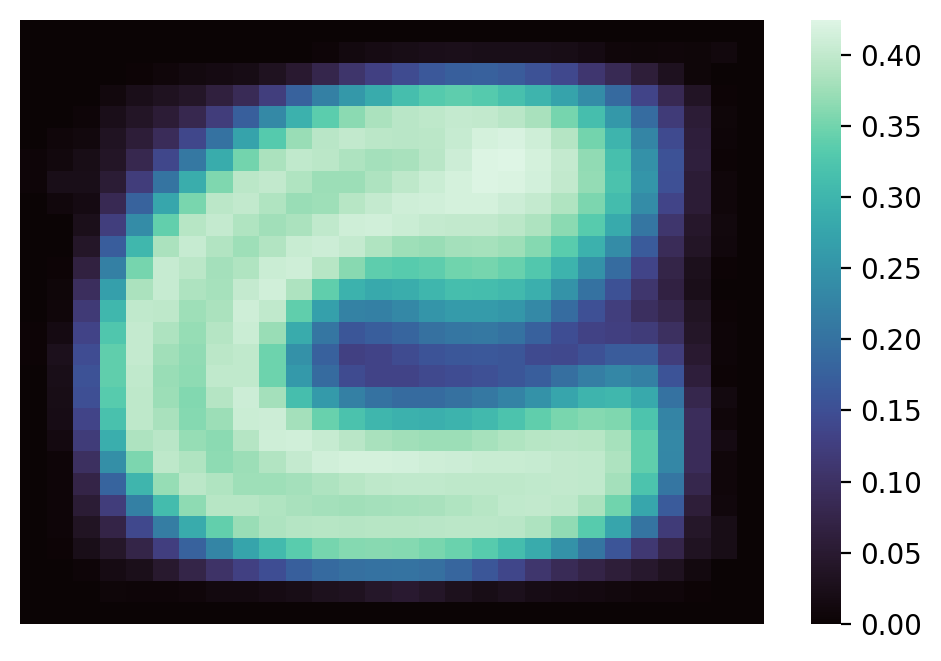
\includegraphics[scale=0.8]{figuras/5a.png}
	\caption{Desviación estándar de cada píxel de la letra C.}
	\label{fig:5a}
\end{figure}

Si realizamos este mismo proceso para cada letra obtenemos los resultados de la Figura \ref{fig:6a}

\begin{figure}[H]
	\centering
	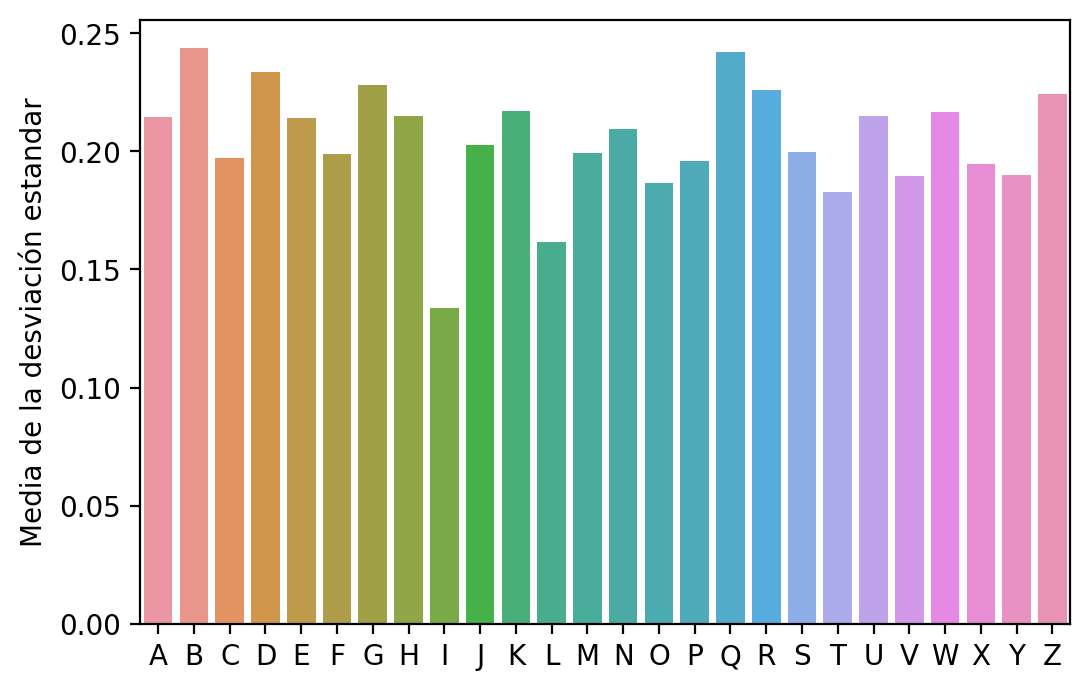
\includegraphics[scale=0.8]{figuras/6a.png}
	\caption{Media de la desviación estándar para cada letra.}
	\label{fig:6a}
\end{figure}

\section{Experimentos realizados}
\subsection{Clasificación binaria}
Para proceder con la tarea de clasificación binaria, fue necesario seleccionar solamente dos clases de todos los datos. Se seleccionaron las letras 'A' y 'L', como se pidió en la consigna.
Como el dataset dado estaba ``limpio'', no hubo ningún obstáculo para conseguir que las partes de datos de entrenamiento y de evaluación (X\_train, X\_test) estuvieran balanceadas.

\begin{itemize}
    \item[]
       \textbf{Experimento 1: Ajuste de un modelo de KNN eligiendo 3 atributos}

En este experimento se ajustó un modelo de K-Nearest Neighbors (KNN) con un valor de cantidad de vecinos igual a 3. 
Para seleccionar los mejores 3 atributos, se hizo un sample de atributos aleatorios que luego fueron evaluados según su desviación estándar (explicación en la introducción). 
Los resultados fueron medidos en exactitud. El mejor resultado nos dio 0.977. Y los mejores atributos fueron: (548, 520, 574) (fig.\ref{fig:7}).

\begin{figure}[H]
	\centering
	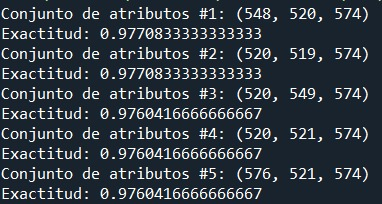
\includegraphics[scale=0.8]{figuras/2a_1.jpg}
	\caption{Los 5 mejores resultados eligiendo 3  atributos}
	\label{fig:7}
\end{figure}
\end{itemize}

\begin{itemize}
    \item[]
       \textbf{Experimento 2: Ajuste de un modelo de KNN eligiendo más atributos}

Para ver si el modelo mejora con más atributos se probó, de forma similar que en el experimento 1, combinar 5 atributos y 10 atributos.
El accuracy mejora un poco con 5 atributos, y en el caso de 10 combinaciones hasta empeora (fig.\ref{fig:8}). Esto puede indicar el overfitting en el modelo.
\begin{figure}[H]
	\centering
	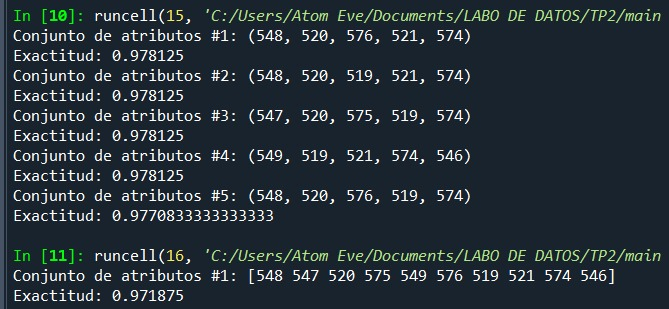
\includegraphics[scale=0.7]{figuras/2a_2.jpg}
	\caption{Exactitudes con combinaciones de 5 atributos y de 10 aributos}
	\label{fig:8}
\end{figure}
\end{itemize}

\begin{itemize}
    \item []
    \textbf{Experimento 3: Ajuste de modelos tomando diferentes valores de k y de combinaciones de atributos}

En este experimento se tomaron diferentes valores de cantidad de vecinos para encontrar el mejor modelo. Se tomaron combinaciones de 5 atributos ya que daba la mejor exactitud. Después de realizar el procedimiento se concluyó que para valores de k entre 3 y 5 el modelo funciona mejor. (fig.\ref{fig:9})

\begin{figure}[H]
	\centering
	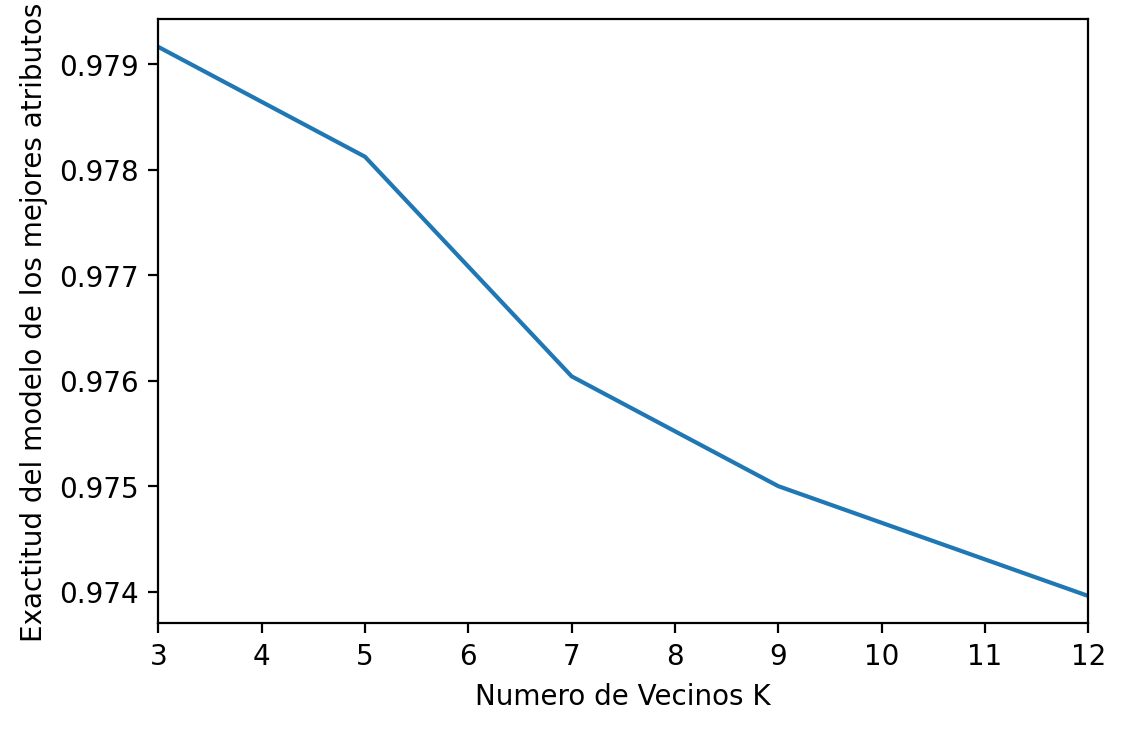
\includegraphics[scale=0.8]{figuras/2e.png}
	\caption{Gráfico de cambio de exactitud del modelo dependiendo de la cantidad de vecinos.}
	\label{fig:9}
\end{figure}

\end{itemize}

\subsection{Clasificación multiclase}
Se cuenta con un modelo de árbol de decisión tal que, dada una imagen, predice a cuál de las vocales ('A', 'E', 'I', 'O', 'U') corresponde. El objetivo de los experimentos descriptos a continuación es seleccionar el mejor modelo que cumpla esta tarea. Para esto se generó un dataframe tomando sólo los datos correspondientes a las letras mencionadas y se los separó en un conjunto de datos de desarrollo (entrenamiento) y otro de validación (held-out). Para reducir el tiempo de ejecución de los experimentos, se tomaron solo los atributos (píxeles de la imagen) considerados más relevantes.

\begin{itemize}
	\item[]
	\textbf{Experimento 1: Ajuste de un modelo de Árbol de Decisión con distintas profundidades}

En este experimento se ajustó un modelo DecisionTreeClassifier variando la profundidad máxima del árbol (max\_depth) desde 1 hasta 21 con incrementos de 2. Se midió la performance del modelo en el conjunto de datos de desarrollo (X\_train).

\begin{figure}[H]
	\centering
	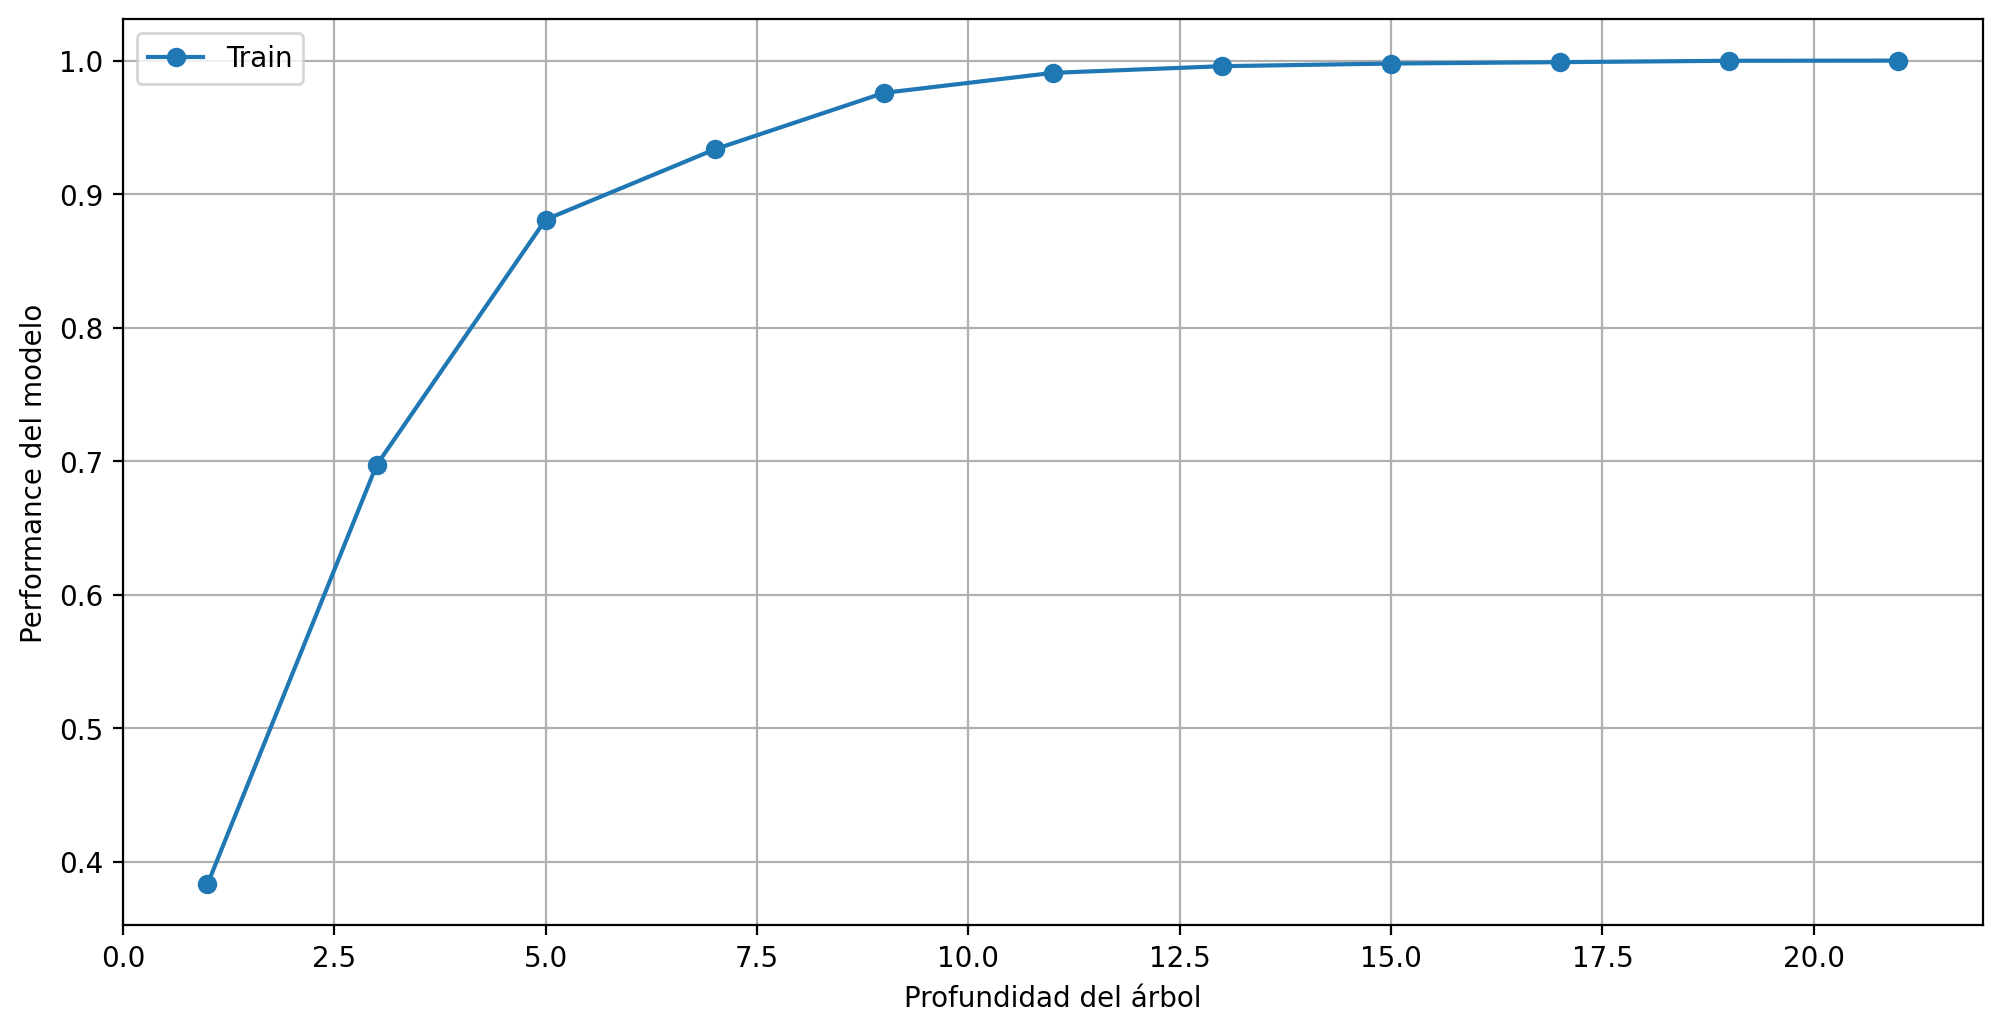
\includegraphics[scale=0.6]{figuras/3b.png}
	\caption{Performance vs profundidad del modelo de árbol de decisión}
	\label{fig:3b}
\end{figure}

Los resultados de este experimento, tal como se ve en la figura \ref{fig:3b}, mostraron que la precisión del modelo aumenta con la profundidad del árbol, lo cual es esperado. Sin embargo, es importante notar que profundidades mayores pueden llevar a sobreajuste (overfitting), donde el modelo aprende demasiado bien los datos de entrenamiento y pierde capacidad de generalización. 

	\item[]
	\textbf{Experimento 2: Validación Cruzada con K-Fold }
 
Con este experimento se buscó encontrar la mejor configuración de hiperparámetros para el modelo. 

A partir del experimento anterior se pudo intuir que para encontrar la profundidad más adecuada, se podían descartar los valores muy bajos (1-6) para evitar el subajuste, y los demasiados altos (mayores a 14) para el sobreajuste. Por esto se optó por variar el hiperparámetro \textit{max\_depth} entre profundidades intermedias. 
Al mismo tiempo, se buscó variar el hiperparámetro \textit{criterion} para obtener la combinación óptima entre profundidad y criterio. 

Se utilizó validación cruzada con KFold (n\_splits=10, shuffle=True, random\_state=1) para evaluar el rendimiento de los modelos DecisionTreeClassifier, en el conjunto de datos de desarrollo (X\_train), con diferentes profundidades máximas del árbol (7 a 14) y criterios de elección de atributos (Gini y Entropy). Una vez obtenidos los distintos valores de performance, separados en datos de entrenamiento y test, por cada \textit{max\_depth} y a su vez, divididos por \textit{criterion}, se tomó el promedio de los scores de performance, resultando en el siguiente gráfico: 

\begin{figure}[H]
	\centering
	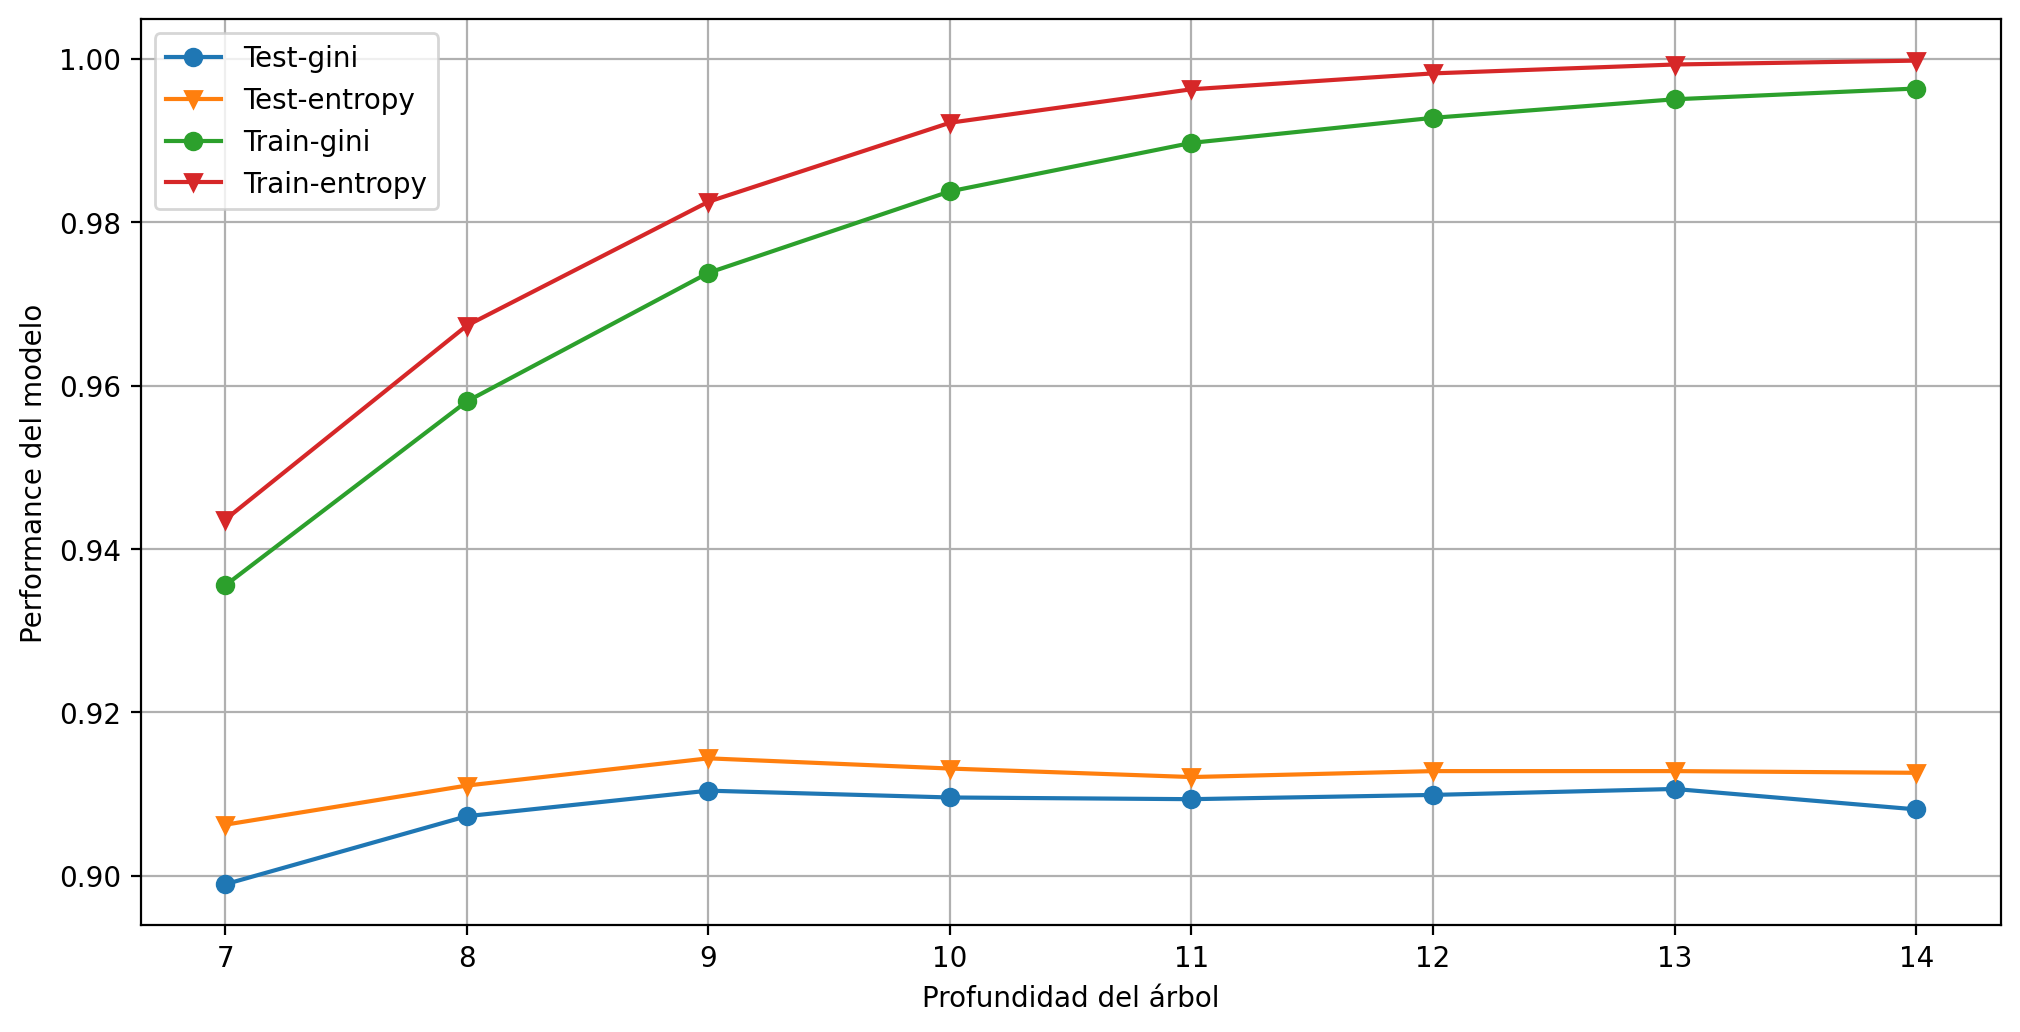
\includegraphics[scale=0.6]{figuras/3c.png}
	\caption{Performance vs profundidad del modelo de árbol de decisión para criterios Gini y Entropy separados en datos de Train y Test}
	\label{fig:3c}
\end{figure}

Como se puede observar en la figura \ref{fig:3c}, los valores de performance en los datos de entrenamiento (Train-gini, Train-entropy) se comportan de forma similar a lo visto en el Experimiento 1, aumentando la precisión del modelo a mayor profundidad del árbol. 
El comportamiento con los datos de test (Test-gini, Test-entropy), indica que la mayor precisión se obtiene con \textit{max\_depth} = 9. Luego de este punto la precisión empieza a disminuir lentamente. 
Con respecto al criterio de elección de atributos, en ambos conjuntos de datos, el más indicado parece ser \textit{criterion} = Entropy.
		
Según este experimento, la mejor combinación de hiperparámetros es con \textit{max\_depth} = 9 y \textit{criterion} = Entropy, obteniendo un promedio de performance de 0.9144.

	\item[]
	\textbf{Experimento 3: Entrenamiento y análisis de performance con el mejor modelo}
	
En el Experimento 2 se determinó que la mejor configuración de hiperparámetros para el modelo es con \textit{max\_depth} = 9 y \textit{criterion} = Entropy. 
Se entrenó entonces a este modelo con todo el conjunto de datos de desarrollo (\texttt{X\_train}) y se lo utilizó para predecir las clases en el conjunto held-out (\texttt{X\_test}). 

A continuación, se muestra la matriz de confusión obtenida:

\begin{table}[H]
    \centering
    \begin{tabular}{c|ccccc}
        & A & E & I & O & U \\
        \hline
        A & 428 & 15 & 8  & 16 & 13 \\
        E & 22  & 433 & 5  & 11 & 9  \\
        I & 3   & 9   & 467 & 0  & 1  \\
        O & 5   & 4   & 0   & 459 & 12 \\
        U & 22  & 6   & 3   & 24 & 425 \\
    \end{tabular}
    \caption{Matriz de confusión del mejor modelo en el conjunto de validación (held-out)}
    \label{tab:matriz_confusion}
\end{table}

Los resultados obtenidos al evaluar el modelo utilizando métricas de performance fueron los siguientes:

\begin{table}[H]
    \centering
    \begin{tabular}{ll}
        \hline
        Métrica    & Valor  \\
        \hline
        Accuracy  & 0.9217 \\
        Precision & 0.9217 \\
        Recall    & 0.9217 \\
        F1        & 0.9217 \\
        \hline
    \end{tabular}
    \caption{Resultados de las métricas de performance del mejor modelo en el conjunto de validación (held-out)}
    \label{tab:resultados}
\end{table}

\end{itemize}


\section{Conclusiones}

A partir de los experimentos realizados, se pueden extraer las siguientes conclusiones:

\begin{itemize}

\item
        Importancia de la reducción de dimensionalidad:

        Se mostró que al aumentar las dimensiones en el modelo, éste se vuelve más complejo y tiende a sufrir de overfitting. Además, al elegir las variables más importantes se puede lograr una mejor performance del modelo.

\item
	Importancia de la profundidad del árbol (\textit{max\_depth}):

	Los experimentos demostraron que aumentar la profundidad del árbol mejora la precisión hasta cierto punto. Sin embargo, profundidades excesivas pueden llevar a sobreajuste, reduciendo la capacidad del modelo para generalizar a nuevos datos.

\item
	Selección del criterio de elección de atributos (\textit{criterion}):

	Se observó que el criterio de Entropy superó ligeramente al criterio de Gini en términos de performance, lo cual fue evidente tanto en el conjunto de entrenamiento como en el conjunto de validación.

\item
	Validación cruzada para elección de hiperparámetros:

	La utilización de validación cruzada con \textit{k-fold} permitió identificar la configuración más adecuada de hiperparámetros que balancea adecuadamente entre precisión y la capacidad de generalización del modelo.  
	La técnica \textit{k-fold} demostró ser una herramienta valiosa para la selección de hiperparámetros.

\item
	Performance del modelo para clasificación multiclase:

	El modelo de árbol de decisión con una profundidad máxima \textit{max\_depth} = 9 y \textit{criterion} = Entropy presentó la mejor configuración de hiperparámetros, logrando un rendimiento promedio de 0.9144 en el conjunto de desarrollo.
	En el conjunto de validación (held-out), este modelo logró un Accuracy, Precision, Recall y F1-Score de 0.9217, indicando una alta capacidad del modelo para generalizar y predecir correctamente las clases de vocales. 

\end{itemize}


\end{document}
